\section{Evaluation}
\subsection{RQ1}
For answering what pooling technique pairs best with each embedding technique, a logistic regression has been performed to test which pooling technique results in the highest accuracy.
However, before we can compare performance, a regularization type needs to be specified. 

\subsubsection{Regularization}

$L_{1}$ and $L_{2}$ regularizations have been tested on our max pooled text embedding techniques, and the results are shown in figure 3.
For all but one of the embeddings, the $L_{2}$ regularization had the upper hand.
That embedding technique, OpenAI's GPT, showed a small advantage when using a $L_{1}$ regularization, however, the difference was very small.
We can conclude that $L_{2}$ regularization works best on most of our models.

\begin{figure}[h]
    \centering
    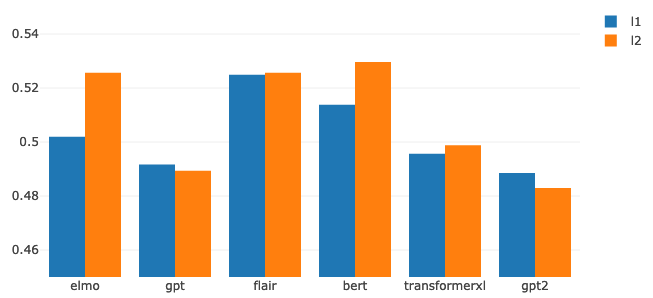
\includegraphics[scale=0.5]{regularizationcomparison}
    \caption{Comparing performance between a $L_{1}$ regularization and a $L_{2}$ regularization on max pooled datasets.}
\end{figure}

\subsubsection{Comparing performance on a logistic regression model}
Now it is clear that the $L_{2}$ regularization performs best on our model, we can compare performance between different pooling strategies.
The results of the classifications are shown in figure 4.
Between the 5 embedding techniques, there was no shared top performing pooling operation. 
For 3 of our embeddings, the max pooling operation resulted in a higher accuracy, while OpenAI's GPT and Flair embeddings gained a higher accuracy with min pooling and average pooling, respectively.

\begin{figure}[t]
    \centering
    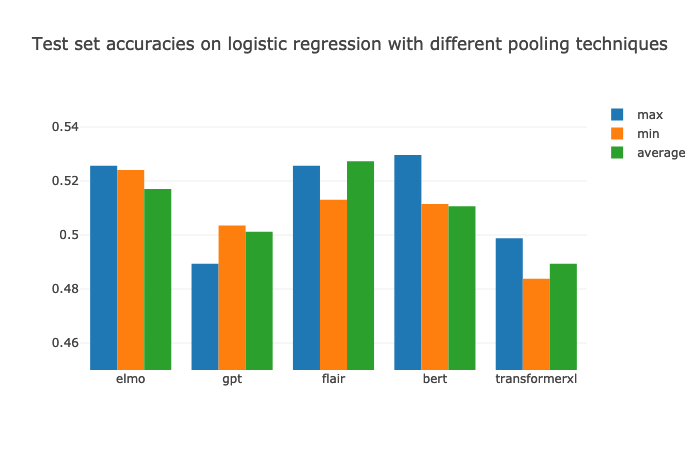
\includegraphics[scale=0.5]{poolingaccuracy}
    \caption{Comparing different pooling strategies.}
\end{figure}

\subsection{RQ2}

\begin{figure}[b!]
    \centering
    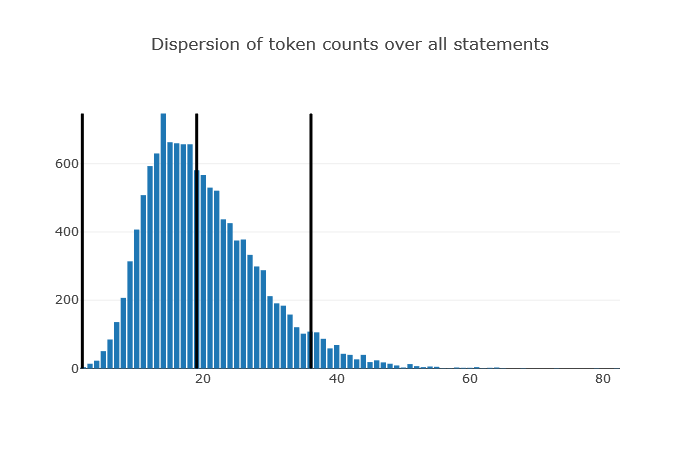
\includegraphics[scale=0.45]{wordlength}
    \caption{Total token counts per statement on the Liar dataset.}
\end{figure}

To find out which sequence length is optimal for neural classification, data with variable amounts of padding has been fed into bidirectional LSTMs and convolutional neural networks.
The lengths between two standard deviations from the median of the total word lengths per statement have been used as a cutoff point, as is illustrated in figure 5. 
This allows the highest cutoff point (\(median + 2 \times \sigma \approx 36\)) to still contain approximately 80\% of the tokens of the longest statement.

\begin{figure}[hbtp]
    \centering
    \begin{subfigure}[b]{1\textwidth}
       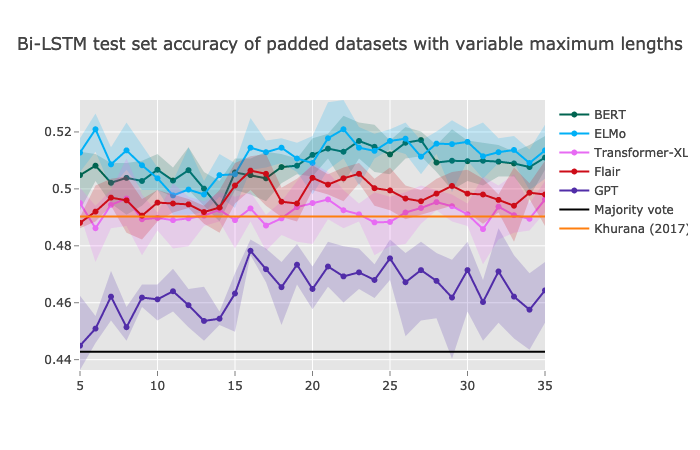
\includegraphics[width=1\linewidth]{bilstmaccuracies}
       \caption{Bidirectional LSTM accuracies.}
    \end{subfigure}
    
    \begin{subfigure}[b]{1\textwidth}
       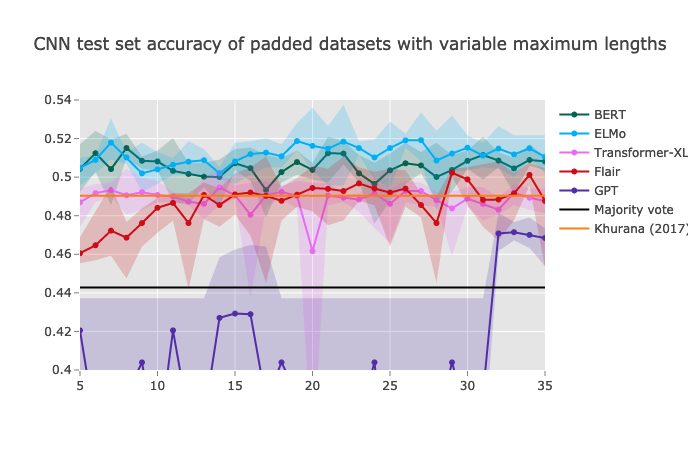
\includegraphics[width=1\linewidth]{cnnaccuracies}
       \caption{Convolutional neural network accuracies.}
    \end{subfigure}
    
    \caption{Test set accuracies with variable maximum lengths over neural network architectures.}
\end{figure}

In figure 6, the accuracies with different amounts of padding can be seen compared to our 3 baselines: Khurana's best score, the majority baseline and our own best score using the doc2vec language model.
In both architectures, performance did not significantly deteriorate or increase, but remained somewhat linear, regardless of how much padding had been inserted.
From this, we can conclude that most of our word embeddings do indeed carry sentence-level context with them.
During training, the whole sentence is taken into account when forming word embeddings, and traces of the whole context are embedded into single word embeddings.
This allows for a stable performance, regardless of how many word embeddings are included in the classification.

The best maximum length seems to lay a litte bit above our average word length of 19, with the top performing model, the ELMo embedding, having an accuracy of 52,09\% on the bi-LSTM architecture with a maximum length of 22.
On the CNN, ELMo embeddings also perform the best, with the best accuracy being 51,92\% when the word embeddings are cutoff at a maximum of 27. 

\subsection{RQ3}
To conclude our search to the best combination of text embeddings with classifiers, performance differences between neural and non-neural classification algorithms have been evaluated.
The results are shown in figure 7. 

\begin{figure}[h]
    \centering
    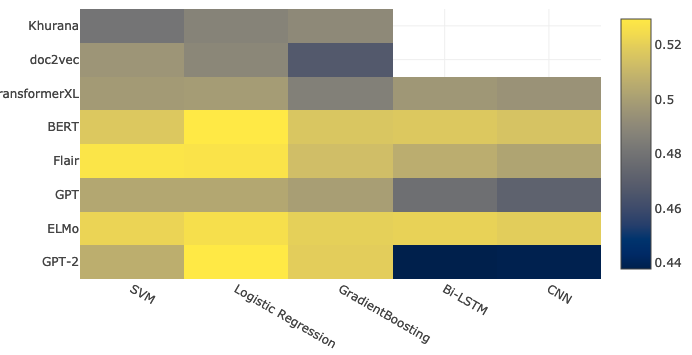
\includegraphics[scale=0.5]{linearvsneural}
    \caption{Comparing different non-neural classifiers with neural classifiers.}
\end{figure}

Clearly, neural architectures either performed worse, or were equal to non-neural classifiers. 
We can conclude that a combination of pre-trained (neural) embedding techniques and regular, non-neural classifiers allow for the best accuracy, as opposed to both a neural embedding and a neural classification architecture.
Of all our tested combinations, a combination of a logistic regression with BERT embeddings performed the best. 
This combination resulted in an accuracy of 52,96\%, almost 4\% better than research conducted by Khurana, 3,4\% better than the best doc2vec combination, and 8,86\% better than the majority baseline.

When applying this combination on the original dataset with 6 labels, an accuracy of 27,51\% has been achieved. 
Research by Wang reached 27\% accuracy without introducing speaker metadata \cite{wang2018}, making the combination of BERT and a logistic regression the best performing classification method at the time of writing.